\section{Experiments}
\label{sec:experiments}
We evaluate SEAL on five simulated and real-world tasks, addressing four questions: (Q1) Can uncertainty-targeted active querying recover guards as accurate as perturbation-based grounding, replacing thousands of oracle-labeled failure rollouts with a handful of safe human demonstrations? (Q2) Does confidence gating reduce false-positive transitions without added latency, relative to a tuned automaton? (Q3) With the localizer learned from safe demonstrations, does the closed-loop system reliably recover from perturbations that drive the state across a guard? (Q4) Does the framework transfer to non-expert users?

Table~\ref{tab:exp_overview} maps tasks to questions. In each task we compare against the strongest baseline available there: GLiDE on the 2D navigation task it defines (where simulated resets and an outcome oracle exist); a hand-tuned automaton on scooping and pick-and-place, where an expert can construct threshold rules on the same features; and open-loop execution on the Robosuite tasks, which isolate reactive recovery. Throughout, \emph{completion time} is the wall-clock time from task start to the terminal mode, \emph{path length} is the accumulated end-effector displacement, and a \emph{false-positive transition} is a gated mode switch triggered by observation noise rather than by an actual change of mode; mIoU measures the overlap between learned and ground-truth mode regions over the workspace.

\begin{table}[t]
\centering
\caption{Overview of the experimental evaluation.}
\label{tab:exp_overview}
\setlength{\tabcolsep}{3.5pt}
\begin{tabular}{lllll}
\toprule
\textbf{Task} & \textbf{Platform} & \textbf{Demos} & \textbf{Baseline} & \textbf{Q} \\
\midrule
2D navigation & sim + FR3 & $6{+}6$ & GLiDE, no-active & Q1, Q3 \\
Wiping & FR3 & $2$ & open-loop & Q3 \\
Lift/Stack & Robosuite & $3{+}4$ & open-loop & Q3 \\
Scooping & FR3 & $4$ & tuned automaton & Q2, Q3 \\
Pick-and-place & FR3 & $2$ & tuned automaton & Q2 \\
Restocking & FR3 + users & $10$ users & unguided demos & Q4 \\
\bottomrule
\end{tabular}
\end{table}

\begin{figure*}[t]
\centering
% TikZ scaffold; panels in Figures/exp_frames/ are crops of the old
% 2d_nav_figure.png -- regenerate from matplotlib with the paper palette
% (seal RGB 0,140,90; glide RGB 200,120,0; tli RGB 80,80,80) for print quality.
\begin{tikzpicture}[font=\small,
  photo/.style={inner sep=0pt}, lbl/.style={font=\scriptsize, align=center}]
\node[photo] (a) {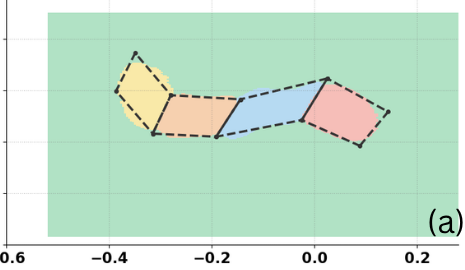
\includegraphics[height=3.0cm]{Figures/exp_frames/nav_guards.png}};
\node[photo, right=4mm of a] (b) {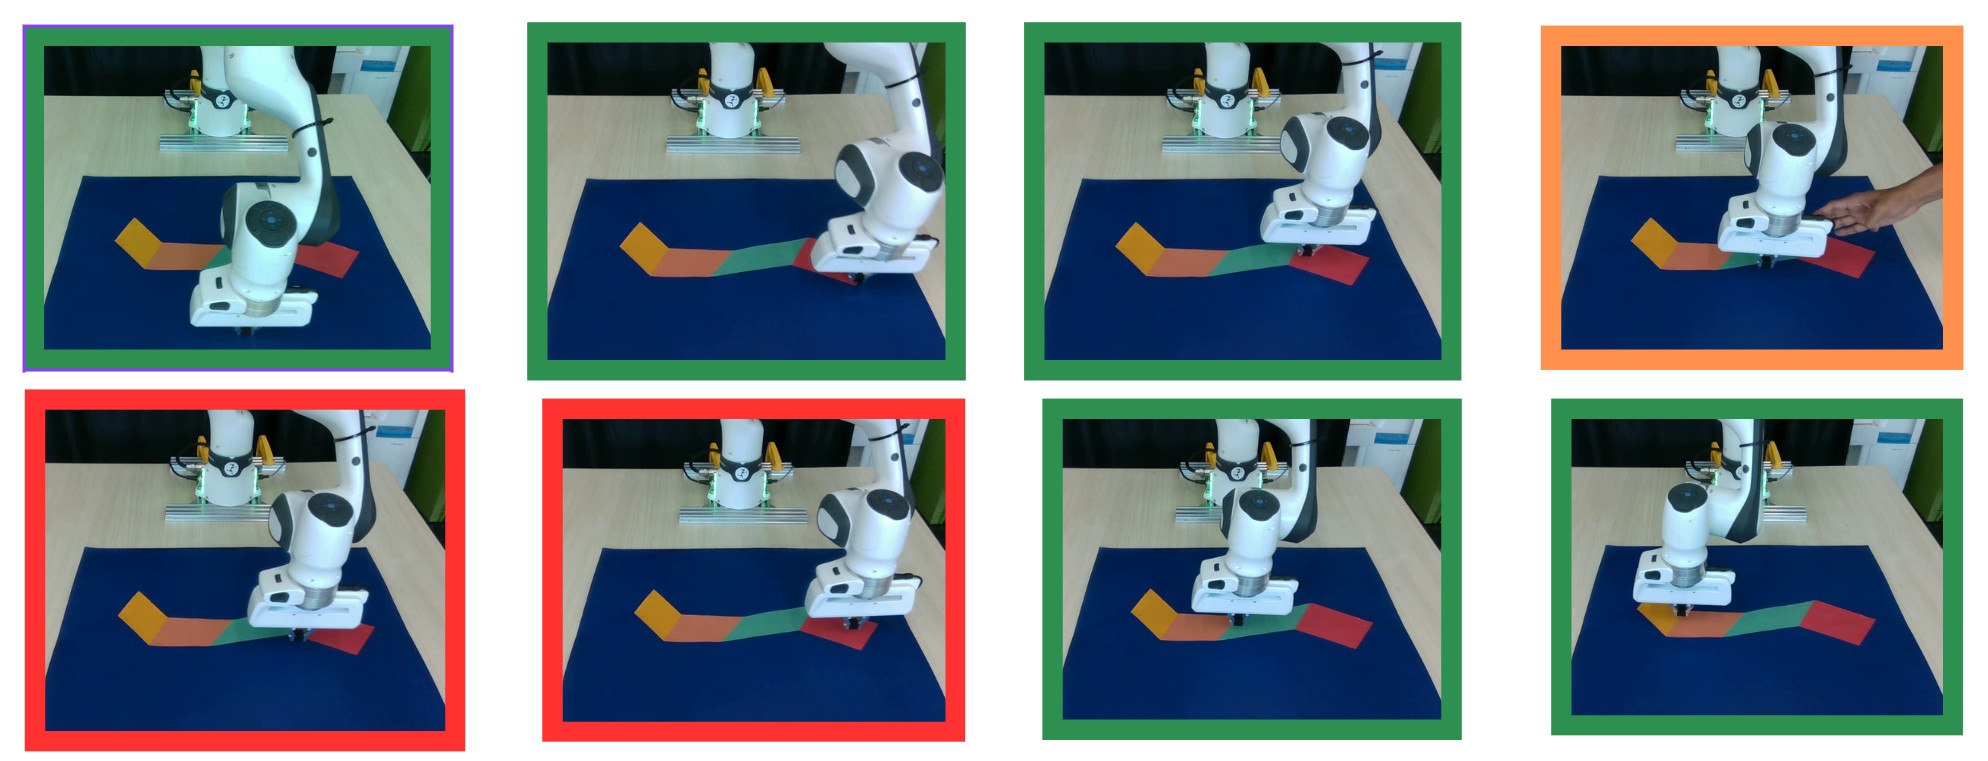
\includegraphics[height=3.0cm]{Figures/exp_frames/nav_episode.png}};
\node[photo, right=4mm of b] (c) {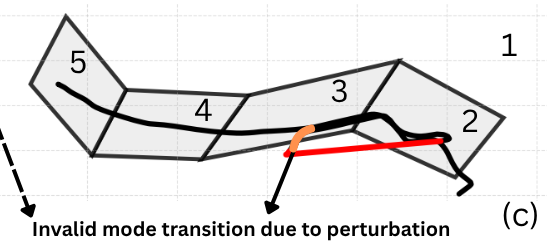
\includegraphics[height=3.0cm]{Figures/exp_frames/nav_traj.png}};
\node[lbl, below=1mm of a] {(a) learned guards (dashed)\\ vs.\ ground-truth regions};
\node[lbl, below=1mm of b] {(b) hardware episode: perturbation\\ (orange frame) and recovery (red frames)};
\node[lbl, below=1mm of c] {(c) executed trajectory over modes;\\ \textcolor{red}{red} = recovery segment};
\end{tikzpicture}

\caption{\textbf{2D navigation on hardware (FR3).} (a) Guards learned from 6+6 demonstrations match the ground-truth mode regions; in this task feature space \emph{is} the workspace, so the guards of Fig.~\ref{fig:seal_ltl_comp} are directly visible. (b) A perturbation drives the state across a non-nominal boundary and the localizer re-engages the correct mode. (c) The perturbation induces an invalid transition; the red segment shows the recovery re-traversal completing the prescribed sequence.}
\label{fig:2d_recovery}
\end{figure*}

\subsection{2D Navigation (Simulation and Hardware)}
\label{sec:2d_nav}
% TODO(fig-consistency): captions/labels now use Fig.-1 language; remaining step is
% regenerating the raster panels (exp_frames/nav_*, cmp_*) from matplotlib with the
% paper palette: seal RGB(0,140,90), glide RGB(200,120,0), tli RGB(80,80,80), and the
% Fig.-1 markers (solid demos, circled queries, dashed queried sub-demos).
Replicated from GLiDE, the task is to traverse colored 2D regions in a prescribed order (Fig.~\ref{fig:comparison}a); here $F_{\min}$ is simply the $(x,y)$ coordinate. We request 6 demonstrations from mode~1 to mode~4 from varied starts, train an initial classifier, select 6 uncertain points, request 6 sub-demonstrations through them, and retrain on the combined 12. As boundary accuracy matters more than labeling the entire space here, we use margin uncertainty. We compare against GLiDE seeded with the same 6 demonstrations and its simulated perturbations.

Fig.~\ref{fig:comparison} shows that SEAL after active querying (b) closely matches the ground truth (a), and clearly improves on the pre-query classifier (c), demonstrating the value of active learning. Table~\ref{tab:miou_results} reports mean Intersection-over-Union (mIoU) against ground truth: SEAL matches GLiDE with 1000 perturbations, while GLiDE degrades sharply as its perturbation budget shrinks. We emphasize the correct accounting of supervision (Q1): GLiDE's perturbations are autonomous and cheap in simulation but require an outcome oracle and a resettable environment, whereas SEAL's additional cost is 6 safe human sub-demonstrations and no oracle; the comparison is thus of \emph{supervision type and safety} (what must exist for each method to run), not of raw sample count or human minutes. Crucially, SEAL never accesses ground-truth labels during training, unlike GLiDE's success oracle. We do not claim to surpass GLiDE, which solves the harder problem of learning from sparse success/failure feedback; we show we can match it with a little more human effort and none of the oracle, perturbation, or reset machinery.
To isolate the impact of uncertainty-targeted selection from the general benefit of acquiring more data, we evaluated a random-query baseline in simulation over $N=10$ randomized seeds. For this ablation we used an algorithmic oracle to provide perfectly segmented demonstrations, which shifts the absolute mIoU scale relative to our human-subject experiments. Starting from identical initial demonstrations, drawing the 6 subsequent queries uniformly at random yielded a mean mIoU improvement of just $+0.07 \pm 0.04$, whereas SEAL's margin-based acquisition drove nearly double the gain, $+0.14 \pm 0.04$. A Wilcoxon signed-rank test on the paired improvements confirms the difference is significant ($W{=}0.0$, $p{=}0.002$, effect size $r{=}1.0$), showing the gains come from identifying classification boundaries rather than demonstration volume alone.

We do not evaluate a history-conditioned (sequence-aware) localizer as a baseline: as argued in Sec.~\ref{sec:supervision}, conditioning on the nominal mode history structurally suppresses the very anomalous transitions a failure monitor must catch.



\begin{figure}[htbp]
\centering
% Crops of the old comparison_GLiDE.png; regenerate with paper palette.
\resizebox{\columnwidth}{!}{%
\begin{tikzpicture}[font=\small,
  photo/.style={inner sep=0pt}, lbl/.style={font=\scriptsize, align=center}]
\node[photo] (gt) {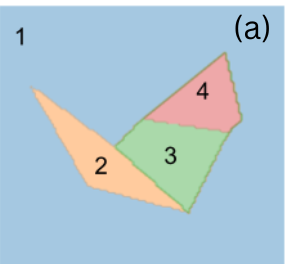
\includegraphics[width=2.05cm]{Figures/exp_frames/cmp_gt.png}};
\node[photo, right=2mm of gt] (s) {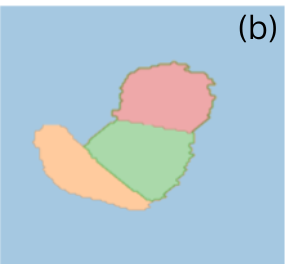
\includegraphics[width=2.05cm]{Figures/exp_frames/cmp_seal.png}};
\node[photo, right=2mm of s] (n) {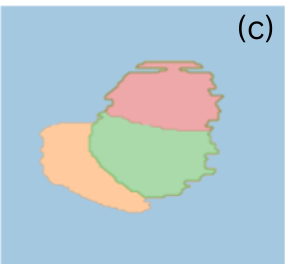
\includegraphics[width=2.05cm]{Figures/exp_frames/cmp_naive.png}};
\node[photo, right=2mm of n] (g) {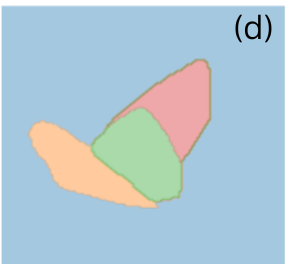
\includegraphics[width=2.05cm]{Figures/exp_frames/cmp_glide.png}};
\node[lbl, below=0.5mm of gt] {(a) ground truth};
\node[lbl, below=0.5mm of s, seal] {(b) SEAL\\ $6{+}6$ demos};
\node[lbl, below=0.5mm of n, seal!60!black] {(c) SEAL, no\\ active round};
\node[lbl, below=0.5mm of g, glide] {(d) GLiDE, $6$ demos\\ ${+}1000$ rollouts};
\end{tikzpicture}%
}

\caption{\textbf{Learned mode regions on 2D navigation.} SEAL with one active round (b) recovers the ground-truth partition (a) as accurately as GLiDE with 1000 oracle-labeled rollouts (d), and markedly better than without the active round (c).}
\label{fig:comparison}
\end{figure}

\begin{table}[h]
    \centering
    \caption{Mean IoU Comparison on 2D Navigation}
    \label{tab:miou_results}
    \begin{tabular}{llc}
        \toprule
        \textbf{Method} & \textbf{Supervision} & \textbf{mIoU} \\
        \midrule
        SEAL (Ours) & 12 safe demos & \textbf{0.82} \\
        GLiDE & 6 demos + 1000 oracle rollouts & 0.80 \\
        SEAL (no active round) & 6 safe demos & 0.73 \\
        GLiDE & 6 demos + 400 oracle rollouts & 0.63 \\
        GLiDE & 6 demos + 100 oracle rollouts & 0.53 \\
        \bottomrule
    \end{tabular}
\end{table}

We replicate the task on a Franka FR3 7-DOF arm with 6+6 demonstrations; Fig.~\ref{fig:2d_recovery} shows the learned guards matching the ground-truth regions on hardware and a full perturbation--recovery episode, in which the localizer re-localizes the perturbed state and completes the prescribed sequence (Q3). Under Assumption~\ref{as:prim} the primitives are mode-invariant and goal-reaching, so on unperturbed rollouts the system follows the nominal guard sequence to completion; the localizer's contribution is to re-establish that sequence after a perturbation drives the state across a boundary.

\subsection{Wiping}
This task evaluates reactive recovery in a continuous, contact-rich setting (Fig.~\ref{fig:compilation}b). A Franka FR3 with an eraser must clean a marker line across three modes (\textit{approach\_align}, \textit{wipe}, \textit{done}), and SEAL trains a supervisor from only 2 demonstrations. We manually applied physical forces to the robot's end-effector during the active wiping motion. The perturbations consisted of either pushing the arm laterally off the planned trajectory, or pushing it upward along the Z-axis to sever contact with the surface and force an incomplete wipe. The open-loop policy fails under perturbation, whereas the SEAL-supervised policy continues to the \textit{done} state, substantially improving the wiped fraction (Fig.~\ref{fig:robosuite_wiping}). Measuring the remaining incomplete path length (out of an initial length of 150), the baseline left an average of $51.75 \pm 15.43$ cm incomplete, whereas SEAL achieved near-perfect recovery, leaving only $4.62 \pm 7.54$ cm incomplete. A Mann-Whitney $U$ test confirmed this improvement is statistically significant ($U=0.0, p=0.0008, r=1.000$). Recovery emerges from localization: path displacement re-localizes \textit{wipe}$\to$\textit{approach\_align}, and incomplete cleaning re-localizes \textit{done}$\to$\textit{approach\_align}.

\begin{figure*}[t]
\centering
% Crops of the old compilation.png (Figures/exp_frames/setup_*.png);
% replace with high-res originals (same filenames) when available.
\resizebox{\textwidth}{!}{%
\begin{tikzpicture}[font=\small,
  photo/.style={inner sep=0pt}, lbl/.style={font=\scriptsize, align=center}]
\node[photo] (s1) {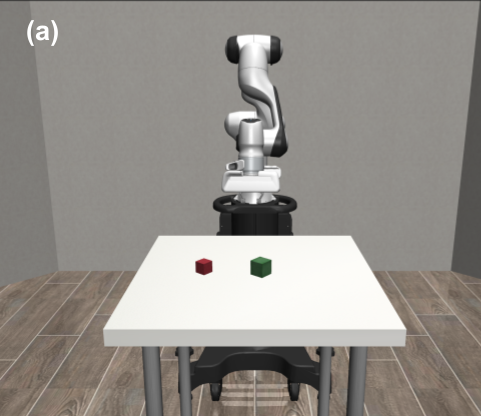
\includegraphics[height=2.9cm]{Figures/exp_frames/setup_stack.png}};
\node[photo, right=2mm of s1] (s2) {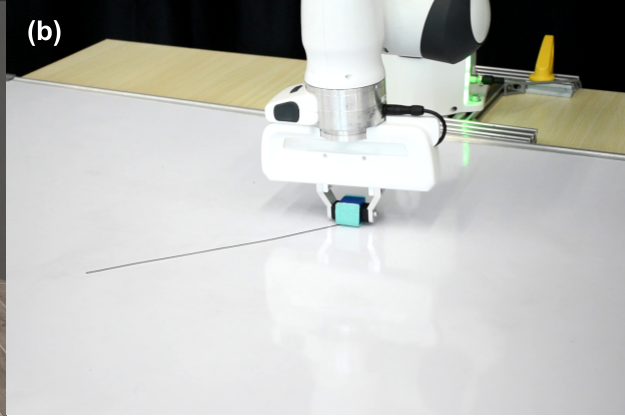
\includegraphics[height=2.9cm]{Figures/exp_frames/setup_wiping.png}};
\node[photo, right=2mm of s2] (s3) {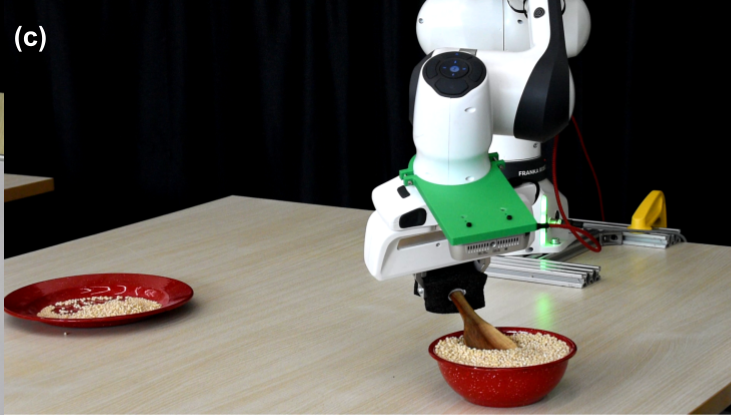
\includegraphics[height=2.9cm]{Figures/exp_frames/setup_scooping.png}};
\node[photo, right=2mm of s3] (s4) {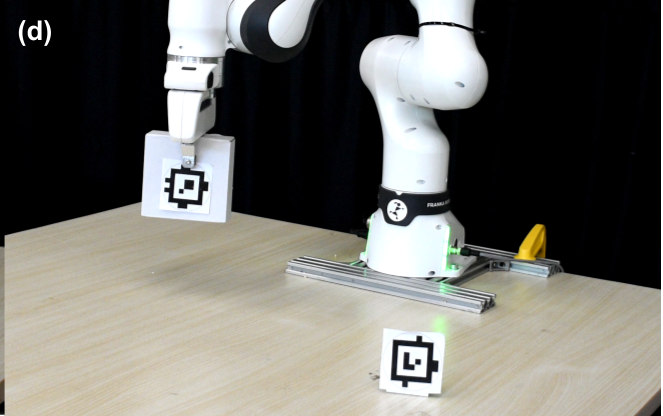
\includegraphics[height=2.9cm]{Figures/exp_frames/setup_pnp.png}};
\node[lbl, below=1mm of s1] {(a) Lift/Stack (Robosuite)};
\node[lbl, below=1mm of s2] {(b) Wiping (Robosuite)};
\node[lbl, below=1mm of s3] {(c) Scooping (FR3)};
\node[lbl, below=1mm of s4] {(d) Pick-and-place (FR3)};
\end{tikzpicture}%
}

\caption{\textbf{Experimental setups} for the four manipulation tasks; the 2D navigation setup is shown in Fig.~\ref{fig:2d_recovery}.}
\label{fig:compilation}
\end{figure*}

\begin{figure}[htbp]
\centering
% Redrawn in pgfplots from the value labels of the old robosuite_wiping.png.
\begin{tikzpicture}
\begin{axis}[
  ybar, bar width=5pt, width=0.97\columnwidth, height=5.2cm,
  ymin=0, ymax=119, ylabel={success rate (\%)},
  symbolic x coords={Wiping,Lift,Stack}, xtick=data,
  enlarge x limits=0.25,
  legend style={at={(0.5,1.02)}, anchor=south, legend columns=4,
                font=\scriptsize, /tikz/every even column/.append style={column sep=3pt}},
  nodes near coords, every node near coord/.append style={font=\tiny, rotate=90, anchor=west},
  tick label style={font=\scriptsize}, label style={font=\scriptsize},
]
\addplot[fill=gray!25, draw=gray!60]  coordinates {(Wiping,100) (Lift,99) (Stack,97)};
\addplot[fill=seal!25, draw=seal!60]  coordinates {(Wiping,100) (Lift,100) (Stack,96)};
\addplot[fill=gray!70, draw=gray]     coordinates {(Wiping,65.6) (Lift,43) (Stack,73)};
\addplot[fill=seal, draw=seal!50!black] coordinates {(Wiping,96.9) (Lift,92) (Stack,90)};
\legend{open-loop (nom.), SEAL (nom.), open-loop (pert.), SEAL (pert.)}
\end{axis}
\end{tikzpicture}

\caption{\textbf{SEAL supervision vs.\ open-loop policies on tasks:} supervision causes no degradation without perturbations (light bars) and substantially mitigates degradation under perturbations (dark bars).}
\label{fig:robosuite_wiping}
\end{figure}

\begin{figure*}[t]
\centering
% Redrawn in pgfplots from the value labels of the old stacking_pnp.png.
% VERIFY against raw data: (i) the first transition-threshold value is assumed
% to be 2 (leftmost point sits left of the "5" tick in the original); (ii) at
% threshold 20 the labels of panels C and D overlap in the original -- values
% used: C automata 1.28 / SEAL 1.28, D automata 37.16 / SEAL 36.87.
\pgfplotsset{exppanel/.style={width=4.65cm, height=3.6cm,
  tick label style={font=\tiny}, label style={font=\tiny},
  title style={font=\scriptsize}, ymajorgrids, grid style={gray!20}}}
\begin{tikzpicture}[font=\small]
\matrix[column sep=2mm, row sep=0mm] {
\begin{axis}[exppanel, ybar, bar width=4.5pt, title={A: Scooping mismatch},
  ylabel={mismatch frames}, symbolic x coords={None,Flicker,Jitter}, xtick=data,
  enlarge x limits=0.3, ymin=0]
\addplot[fill=glide, draw=glide!50!black, error bars/.cd, y dir=both, y explicit] 
  coordinates {(None,68.67) +- (0,41.63) (Flicker,97.33) +- (0,17.50) (Jitter,127.50) +- (0,16.78)};
\addplot[fill=seal, draw=seal!50!black, error bars/.cd, y dir=both, y explicit] 
  coordinates {(None,0.00) +- (0,0.00) (Flicker,38.33) +- (0,5.51) (Jitter,27.25) +- (0,20.07)};
\end{axis} &
\begin{axis}[exppanel, title={B: Scooping transitions}, ylabel={total transitions},
  xlabel={transition threshold}, xtick={2,5,10,20}, ymin=0]
\addplot[glide, thick, mark=square*, error bars/.cd, y dir=both, y explicit] 
  coordinates {(2,13.00) +- (0,0.00) (5,5.67) +- (0,3.06) (10,6.33) +- (0,4.16) (20,3.00) +- (0,0.00)};
\addplot[seal, thick, mark=*, error bars/.cd, y dir=both, y explicit] 
  coordinates {(2,3.00) +- (0,0.00) (5,3.00) +- (0,0.00) (10,3.00) +- (0,0.00) (20,3.00) +- (0,0.00)};
\end{axis} &
\begin{axis}[exppanel, title={C: Scooping path length}, ylabel={path length (m)},
  xlabel={transition threshold}, xtick={2,5,10,20}]
\addplot[glide, thick, mark=square*, error bars/.cd, y dir=both, y explicit] 
  coordinates {(2,1.40) +- (0,0.00) (5,1.41) +- (0,0.12) (10,1.44) +- (0,0.21) (20,1.28) +- (0,0.00)};
\addplot[seal, thick, mark=*, error bars/.cd, y dir=both, y explicit] 
  coordinates {(2,1.27) +- (0,0.00) (5,1.27) +- (0,0.00) (10,1.28) +- (0,0.01) (20,1.28) +- (0,0.00)};
\end{axis} &
\begin{axis}[exppanel, title={D: Scooping completion time}, ylabel={time (s)},
  xlabel={transition threshold}, xtick={2,5,10,20}]
\addplot[glide, thick, mark=square*, error bars/.cd, y dir=both, y explicit] 
  coordinates {(2,42.98) +- (0,0.00) (5,40.44) +- (0,3.97) (10,42.59) +- (0,8.44) (20,37.16) +- (0,1.57)};
\addplot[seal, thick, mark=*, error bars/.cd, y dir=both, y explicit] 
  coordinates {(2,37.25) +- (0,0.00) (5,37.25) +- (0,0.96) (10,36.55) +- (0,0.29) (20,36.87) +- (0,0.60)};
\end{axis} \\
\begin{axis}[exppanel, ybar, bar width=6pt, title={E: P\&P mismatch},
  ylabel={mismatch frames}, symbolic x coords={Nominal,Perturbed}, xtick=data,
  enlarge x limits=0.5, ymin=0]
\addplot[fill=glide, draw=glide!50!black, error bars/.cd, y dir=both, y explicit] 
  coordinates {(Nominal,49.00) +- (0,25.36) (Perturbed,151.14) +- (0,149.75)};
\addplot[fill=seal, draw=seal!50!black, error bars/.cd, y dir=both, y explicit] 
  coordinates {(Nominal,17.60) +- (0,13.13) (Perturbed,56.57) +- (0,33.83)};
\end{axis} &
\begin{axis}[exppanel, ybar, bar width=6pt, title={F: P\&P transitions},
  ylabel={total transitions}, symbolic x coords={Nominal,Perturbed}, xtick=data,
  enlarge x limits=0.5, ymin=0]
\addplot[fill=glide, draw=glide!50!black, error bars/.cd, y dir=both, y explicit] 
  coordinates {(Nominal,4.67) +- (0,1.15) (Perturbed,12.71) +- (0,8.88)};
\addplot[fill=seal, draw=seal!50!black, error bars/.cd, y dir=both, y explicit] 
  coordinates {(Nominal,4.00) +- (0,0.00) (Perturbed,8.00) +- (0,2.77)};
\end{axis} &
\begin{axis}[exppanel, ybar, bar width=6pt, title={G: P\&P path length},
  ylabel={path length (m)}, symbolic x coords={Nominal,Perturbed}, xtick=data,
  enlarge x limits=0.5, ymin=0]
\addplot[fill=glide, draw=glide!50!black, error bars/.cd, y dir=both, y explicit] 
  coordinates {(Nominal,1.54) +- (0,0.34) (Perturbed,3.01) +- (0,1.65)};
\addplot[fill=seal, draw=seal!50!black, error bars/.cd, y dir=both, y explicit] 
  coordinates {(Nominal,1.40) +- (0,0.23) (Perturbed,2.47) +- (0,0.89)};
\end{axis} &
\begin{axis}[exppanel, ybar, bar width=6pt, title={H: P\&P completion time},
  ylabel={time (s)}, symbolic x coords={Nominal,Perturbed}, xtick=data,
  enlarge x limits=0.5, ymin=0]
\addplot[fill=glide, draw=glide!50!black, error bars/.cd, y dir=both, y explicit] 
  coordinates {(Nominal,33.96) +- (0,4.22) (Perturbed,68.81) +- (0,35.88)};
\addplot[fill=seal, draw=seal!50!black, error bars/.cd, y dir=both, y explicit] 
  coordinates {(Nominal,35.90) +- (0,16.50) (Perturbed,55.72) +- (0,21.91)};
\end{axis} \\
};
\node[anchor=north, font=\scriptsize] at (current bounding box.south)
  {\textcolor{glide}{$\blacksquare$} tuned automaton \quad \textcolor{seal}{$\blacksquare$} SEAL \quad (lower is better in all panels)};
\end{tikzpicture}
\caption{\textbf{Comparison with tuned automata.} Scooping (A--D): confidence-gated transitions eliminate false positives as the transition threshold shrinks, yielding fewer spurious transitions, shorter paths, and faster completion. Pick-and-place (E--H): SEAL improves all efficiency metrics under both nominal and perturbed conditions.}
\label{fig:scooping_pnp}
\end{figure*}

\subsection{Block Lifting and Stacking (Robosuite)}
We test non-monotonic features in the Lift and Stack environments~\cite{robosuite2020} (Fig.~\ref{fig:compilation}a). Gripper width is mapped to a binary \textit{grasped} feature to handle its non-monotonic profile, and relative end-effector-to-cube distances complete $F_{\min}$; SEAL trains on 7 demonstrations (3 nominal + 4 active) with separate continuous boundaries per gripper status, a case where the mixed-feature product kernel is useful. Over 100 episodes under random gripper perturbations (a 1\% per-step chance of the gripper opening and staying open for 5 control steps), SEAL maintains a near-perfect nominal success rate and dramatically mitigates degradation under perturbation relative to open-loop (Fig.~\ref{fig:robosuite_wiping}).

\subsection{Scooping}
\label{sec:scooping}
We adopt GLiDE's scooping task (Fig.~\ref{fig:compilation}c): scoop, transport, and deposit rice from a bowl to a plate using a spoon on the end-effector. Open-loop execution fails at the task level if rice spills during transport or scooping fails, a case where failure demonstrations are hard to reset and self-supervised data collection is infeasible, so GLiDE cannot be run here. We detect grains on the spoon with a wrist camera (a binary feature) and use relative end-effector-to-bowl and -plate positions, training with 4 demonstrations.

Beyond comparison to open-loop, we ask how SEAL compares to a tuned automaton with expert-set thresholds: effectively an ideal, hand-built localizer that a learned classifier can only approximate but that is far harder to construct. We design and tune such an automaton on the same features. Because feature and prediction noise is unavoidable, especially near boundaries, \emph{all} classifiers, designed or learned, must confirm a switch over a small buffer to avoid false positives, trading latency against robustness. SEAL breaks this trade (Q2): with access to prediction confidence, it keeps a very small dwell and instead rejects low-confidence switches, smoothing boundary jitter; a genuine perturbation pushes the state deep into another region where confidence is high, giving a fast response. Thus SEAL attains low latency and low false-positive rate simultaneously. Note this reconciles the two roles of the automaton in our narrative: it is an accurate localizer, yet brittle to observation noise precisely because it lacks a calibrated confidence to gate on.

To evaluate continuous performance metrics during the scooping task under adversarial noise, we conducted paired trials ($n=10$, pooling nominal, flicker, and jitter conditions) to compare the tuned automaton against SEAL.

SEAL significantly outperformed the baseline across all continuous trajectory metrics. It completed the task faster ($37.03 \pm 0.67$\,s vs $40.92 \pm 4.86$\,s; $W{=}4.0$, $p{=}0.0137$, $r{=}0.855$) and followed a more efficient trajectory, minimizing unnecessary spatial deviations ($1.28 \pm 0.01$\,m vs $1.38 \pm 0.13$\,m; $W{=}1.0$, $p{=}0.0039$, $r{=}0.964$). Crucially, SEAL suppressed state chattering: the automaton suffered an average of $3.60 \pm 3.98$ false-positive transitions per trial, while SEAL incurred $0.00 \pm 0.00$ ($W{=}0.0$, $p{=}0.0312$, $r{=}1.0$).

The perturbation strategy was as follows: "Flicker" noise applied a 20\% uniform probability per step of dropping the detected grain count to zero, while "Jitter" noise injected Gaussian noise $\mathcal{N}(0, 0.06)$ meters into the continuous distance estimates for the bowl and target. The transition persistence thresholds $\{2, 5, 10, 20\}$ were specifically chosen to demonstrate a critical latency trade-off: while high thresholds (e.g., 20) allow classical automata to filter noisy observations at the cost of reactivity, the probabilistic SEAL framework achieves reliable, rapid recovery at the lowest latencies without needing those high step delays.
 
 Both policies complete every unperturbed trial. Under Assumption~\ref{as:prim} the primitives are mode-invariant and goal-reaching, so the relevant question (Q3) is whether the learned localizer honors exactly the nominal guard sequence rather than injecting spurious crossings: the nominal transition counts in Fig.~\ref{fig:scooping_pnp}B,F (three and four for SEAL) confirm it does.
 
 
 However, as the threshold shrinks, SEAL incurs no false-positive transitions while those of the automaton rise (Fig.~\ref{fig:scooping_pnp}B), giving the automaton significantly higher completion times (Fig.~\ref{fig:scooping_pnp}D) and longer paths (Fig.~\ref{fig:scooping_pnp}C). As with any learned model, SEAL's accuracy depends on demonstration quality; a classifier trained on poor data cannot outperform a tuned automaton even with confidence gating. We do not report a time-indexed OOD detector (e.g., an Eiband-style GMM~\cite{eiband_intuitive_2019}) as a baseline here: such a detector only flags anomalies rather than recovering from them, is sensitive to execution-speed differences between demonstrations and test (flagging a merely slower or faster success as a failure), and does not naturally admit discrete features, consistent with the spatial-generalization limitation discussed in Sec.~\ref{sec:related}.{\color{blue}\ [INTERNAL, discuss: we also ran this baseline in preliminary trials and it performed poorly; add ``(not shown)'' here only if we are comfortable asserting an unpublished negative result.]}

\subsection{Pick and Place}
The robot picks a box and places it near a target (Fig.~\ref{fig:compilation}d), both tracked with AprilTags~\cite{7759617} and a RealSense D435i. With gripper pick-and-place motions the base success rate is lower and failure demonstrations (object falling from the gripper) are potentially unsafe. We divide the task into \textit{Pick}, \textit{Transport}, \textit{Place}, and \textit{Retreat}, each with an object-conditioned primitive, and train from 2 demonstrations using relative distances and a binary gripper state.

To evaluate the framework's capacity to handle physical disturbances, we conducted 41 real-world pick-and-place trials, comparing SEAL against the open-loop automaton under both nominal ($n=21$) and manually perturbed ($n=20$) conditions. The perturbation protocol involved actively moving target objects, blocking the gripper, or dislodging the payload mid-transport. Because manually induced physical perturbations cannot be perfectly replicated across trials, the runs constitute independent samples; we therefore isolate the successfully completed trials and evaluate continuous metrics using the non-parametric Wilcoxon rank-sum (Mann-Whitney $U$) test, discarding failed runs (which occurred at similar rates for both approaches).

On the nominal runs, SEAL matched the baseline's kinematics (no significant difference in completion time or path length, $p > 0.39$, $r \le 0.467$), showing the probabilistic layer does not impede standard operation. SEAL also preserved the nominal task topology, executing exactly 4 transitions across all nominal trials ($4.00 \pm 0.00$), whereas the baseline averaged $4.67 \pm 1.15$, indicating that rigid heuristic thresholds cause false-positive state shifts even without external perturbations. SEAL further showed a strong trend, though not statistically significant, toward reducing internal state-disagreement frames ($17.60 \pm 13.13$ vs $49.00 \pm 25.36$; $U{=}1.0$, $p{=}0.071$, $r{=}0.867$).

Under perturbed conditions, SEAL's structural stability became critical. While high variance in manual perturbations prevented significance for discrete transitions ($U{=}16.0$, $p{=}0.274$, $r{=}0.347$), SEAL bounded recovery chattering tightly ($8.00 \pm 2.77$ transitions, maximum 13), whereas the baseline suffered severe state oscillation with outliers up to 31 transitions ($12.71 \pm 8.88$). SEAL again showed a strong trend toward suppressing state-estimation mismatches ($56.57 \pm 33.83$ vs $151.14 \pm 149.75$; $U{=}10.0$, $p{=}0.073$, $r{=}0.592$). Because the automaton accumulates far higher disagreement, it must rely on large temporal buffers to prevent runaway mode switching; at smaller buffers it would suffer many more false transitions than SEAL.

Finally, while SEAL yielded faster and shorter recovery trajectories (e.g., $55.72 \pm 21.91$\,s vs $68.81 \pm 35.88$\,s), the variance of human-applied perturbations left these kinematic differences short of significance ($p > 0.45$, $r \le 0.265$). Here we fix the transition threshold and instead vary start and goal positions to test generalization.
%%%%%%%%%%%%%%%%%%%%%%%%%%%%%%%%%%%%%%%%%%%%%%%%%%%%%%%%%%%%%%%%%%%%%%%%%%%%%%%%
